
\documentclass[12pt]{article}
\pdfpagewidth 8.5in
\pdfpageheight 11in
\usepackage{fullpage,graphicx,amsmath,sidecap,url, setspace, mathtools,wrapfig,textcomp,bm,amssymb} % url included for bibtex to be happy
\usepackage[hang,small,bf]{caption}
\usepackage[top=1in, bottom=0.95in, left=0.75in, right=0.75in]{geometry}
\usepackage{indentfirst}
\usepackage{gensymb,multicol}
\usepackage[T1]{fontenc}

\usepackage[backend=bibtex, style=authoryear-icomp, sortlocale=de_DE, natbib=true, url=false, doi=true, eprint=false]{biblatex}
\addbibresource{RefBib.bib}
\renewcommand*{\bibfont}{\footnotesize}
\renewbibmacro{in:}{}
\AtEveryBibitem{\clearfield{title}}

%\lhead{\# 13}
%\title{\textbf{The Fun}}
%\author{\text{ID: 13}}
%\date{}
\begin{document}
\setcounter{page}{1}
\pagenumbering{arabic}
%\maketitle
\centering \LARGE \textbf{Probing the Fundamental Plane of Black Hole Activity in the Illustris Simulation}

\small Cool People Names

\abstract 
\singlespacing 
STUFF STUFF STUFF STUFF STUFF STUFF STUFF STUFF STUFF STUFF STUFF STUFF STUFF STUFF STUFF STUFF STUFF STUFF STUFF STUFF STUFF STUFF STUFF STUFF STUFF STUFF STUFF STUFF STUFF STUFF STUFF STUFF STUFF STUFF STUFF STUFF STUFF STUFF STUFF STUFF STUFF STUFF STUFF STUFF STUFF STUFF STUFF STUFF STUFF STUFF STUFF STUFF STUFF STUFF STUFF STUFF STUFF STUFF STUFF STUFF STUFF STUFF STUFF STUFF STUFF STUFF 

\singlespacing
\section{Introduction}
\subsection{Black Hole Properties in the Illustrious Simulation}
Accreting black holes (BHs) such as active galactic nuclei (AGN) are believed to be important in the evolution of galaxies as the feedback from AGN can trigger and/or quench star formation. Thus, in order to understand galaxy evolution, it is important to understand the physics of BH. Specifically, it's important to probe the BH's influence on its surrounding environment.

There are distinctive signatures of BH activity that can be used to probe the existence of BH. For example, relativistic jets emitting synchrotron radiation in the radio band are one signature. Strong X-ray emission from from inverse-Compton scattering in the corona can be related to the accretion flow of the BH. In 2003, Merloni et. al  investigated the properties of $\sim$100 AGN's compact emission in the X-ray and radio bands and showed that the radio luminosity is correlated with both the mass and the X-ray luminosity at a highly significant level. These sources defined a fundamental plane in the three-dimensional space as shown in Figure \ref{FP}. The fundamental plane (FP) suggests that the physical processes regulating the conversion of an accretion flow into radiative energy could be universal across the entire black hole mass scale \cite{Merloni2003}. The FP is defined as

\begin{equation}
\log L_R=0.6 \log L_x+0.78 \log M+7.33
\end{equation}
, where the radio luminosity is $L_R$, the X-ray luminosity is $L_X$, and the mass of the BH is $M$.Then from the FP, the accretion-powered X-ray luminosity can be expressed as,
\begin{equation}
\log L_x = \log M+q \log \dot{m}+K_2
\label{LxFP}
\end{equation}
, where $K_2$ is normalization constant. Depending on the accretion flow model, the efficiency coefficient $q$ ranges from 0.5 (optically thick thin disk accretion flow) to 2.3 (advection dominated accretion flow). The most significant aspect of the FP is that it is a correlation which we can apply our general knowledge of galactic BHs to AGNs and vice versa.

\begin{figure}
\centering
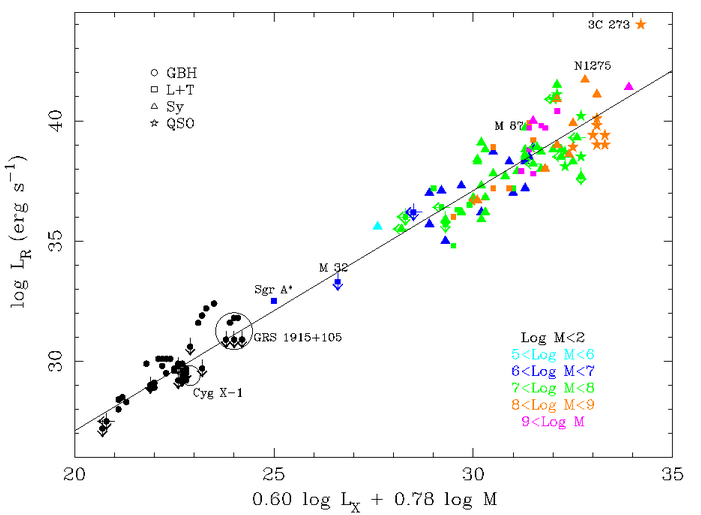
\includegraphics[width=13.5cm]{FP.png}
\caption{Edge-on view of the fundamental plane given by the BH mass, radio luminosity, and X-ray luminosity. \cite{Merloni2003} \label{FP}}
\end{figure}

\subsection{Black Holes in the Illustris Simulation}
The Illustris Project is a series of large-scale cosmological hydrodynamical simulations of galaxy formation \cite{Vogelsberg2014}. The simulation consists of large cosmological situations in a periodic box with 106.5 Mpc, simulated with different physics at different resolutions. It assumes a standard flat $\Lambda$CDM cosmology with $\Omega_{m,0}=0.2726$, $\Omega_{\Lambda,0}=0.72746$, $\Omega_{b,0}=0.0456$, and $H_{0}=70.4$ km s$^{-1}$ Mpc$^{-1}$ from the Wilkinson Microwave Anisotropy Probe 9-year data realease \cite{Hinshaw2013}. 

In the Illustris simulations, collision-less black hole particles with a seed mass of $1.42 \times 10^5 M_\odot$ are placed in dark matter halos of mass greater than $7.1 \times 10^10 M_\odot$ \cite{Sijacki2014}.  The black hole seeds are allowed to grow through gas accretion or through mergers with other black holes.  At $z=0$, there are 32,542 black holes in total with 3965 black holes more massive than $10^7 M_\odot$ \cite{Sijacki2014}. 

In our project, we aim to reproduce the fundamental plane of black hole activity in the Illustris Project to see how well the BHs in the simulation fit with observations. Most specifically, we aim to determine the efficiency coefficient $q$ in Equation \ref{LxFP} in the Illustris simulation using the mass and mass accretion rates of BHs. From this analysis, we can begin to understand to how well the Illustris simulates the real physics of black holes in the universe.

This paper is structured as follows. In Section 2, we outline our methodology. In Section 3, we discuss our results. In Section 4. we examine how well Illustris simulates the physics of black hole in our discussion. 


\printbibliography
\end{document}